\chapter{Общие положения}

\hspace*{1.25cm}Данная глава посвящена формальной постановке задачи предиктивного анализа задержек в конвейере видеоаналитики и представлению архитектуры исследуемой системы. В рамках главы вводятся ключевые математические обозначения, определяются целевые метрики и ограничения, формулируются требования к разрабатываемому алгоритму. Особое внимание уделяется описанию структуры видеоконвейера и точек сбора телеметрических данных, которые лягут в основу построения прогностической модели.

\section{Архитектура системы видеоаналитики}

\hspace*{1.25cm}Исследуемая система видеоаналитики представляет собой многокомпонентный конвейер, предназначенный для обработки видеопотоков в режиме реального времени с применением алгоритмов компьютерного зрения для детекции событий и объектов. Архитектура системы строится по принципу микросервисной архитектуры, что обеспечивает масштабируемость и отказоустойчивость, но одновременно усложняет задачи мониторинга и диагностики производительности.

\hspace*{1.25cm}Видеоконвейер включает следующие основные компоненты: модуль захвата видеопотока с IP-камер (получающий данные по протоколу RTSP), ML-pipeline для применения алгоритмов компьютерного зрения, брокер сообщений Apache Kafka [4] для асинхронной передачи результатов обработки, бэкенд-сервисы для бизнес-логики и сохранения данных, а также WebSocket-клиенты для доставки уведомлений конечным пользователям. Каждый компонент генерирует множество метрик производительности, которые собираются централизованной системой мониторинга Prometheus [2].

\hspace*{1.25cm}Критической характеристикой системы является end-to-end-задержка, измеряемая как время от момента возникновения события в видеопотоке до его отображения на интерфейсе оператора. Данная метрика, обозначаемая как $common\_event\_delay$, напрямую влияет на эффективность работы операторов и качество принимаемых ими решений в критических ситуациях.

\section{Постановка задачи}

\hspace*{1.25cm}Для формальной постановки задачи прогнозирования введем необходимые математические обозначения и определения.

\subsection*{Дано}
\begin{enumerate}
	\item \textbf{Многомерный временной ряд} метрик, собираемых из системы мониторинга Prometheus с периодом дискретизации 15 секунд. В каждый момент времени $t_i$ фиксируется $d$-мерный вектор наблюдений $\mathbf{x}_i = [m^{(1)}_i, \dots, m^{(d)}_i] \in \mathbb{R}^d$, характеризующий состояние видеоконвейера. Объем доступных исторических данных составляет 90643 точки за 16 дней.
	\item \textbf{Горизонт прогнозирования} $\Delta = 900$ временных шагов, что соответствует 3.75 часам.
\end{enumerate}

\subsection*{Найти}
\begin{enumerate}
	\item \textbf{Целевую функцию} $f^*: \mathbb{R}^{L \times d} \to \mathbb{R}$, которая отображает историю наблюдений (представленную матрицей $X_k \in \mathbb{R}^{L \times d}$ из $L$ последних векторов наблюдений) в будущее значение целевой метрики \\
	$y_k = common\_event\_delay(t_k + \Delta)$.
	\item \textbf{Прогностический алгоритм} $A(X_k)$, который является наилучшей аппроксимацией целевой функции $f^*$.
\end{enumerate}

\subsection*{Критерии качества и ограничения}
\hspace*{1.25cm}Разрабатываемый алгоритм $A$ должен удовлетворять следующим требованиям:
\begin{enumerate}
	\item \textbf{Точность прогнозирования:} средняя абсолютная процентная ошибка (MAPE) на тестовых данных должна быть менее 10\%.
	\item \textbf{Производительность:} время вычисления одного прогноза (inference time) на целевом оборудовании не должно превышать 5 секунд.
	\item \textbf{Интерпретируемость:} модель должна предоставлять возможность оценить важность признаков, влияющих на прогноз.
	\item \textbf{Практичность:} решение должно быть реализовано в виде, пригодном для интеграции в существующий MLOps-конвейер, включая контейнеризацию с помощью Docker.
\end{enumerate}

\begin{landscape}
\vspace*{\fill}
\begin{figure}[H]
	\centering
	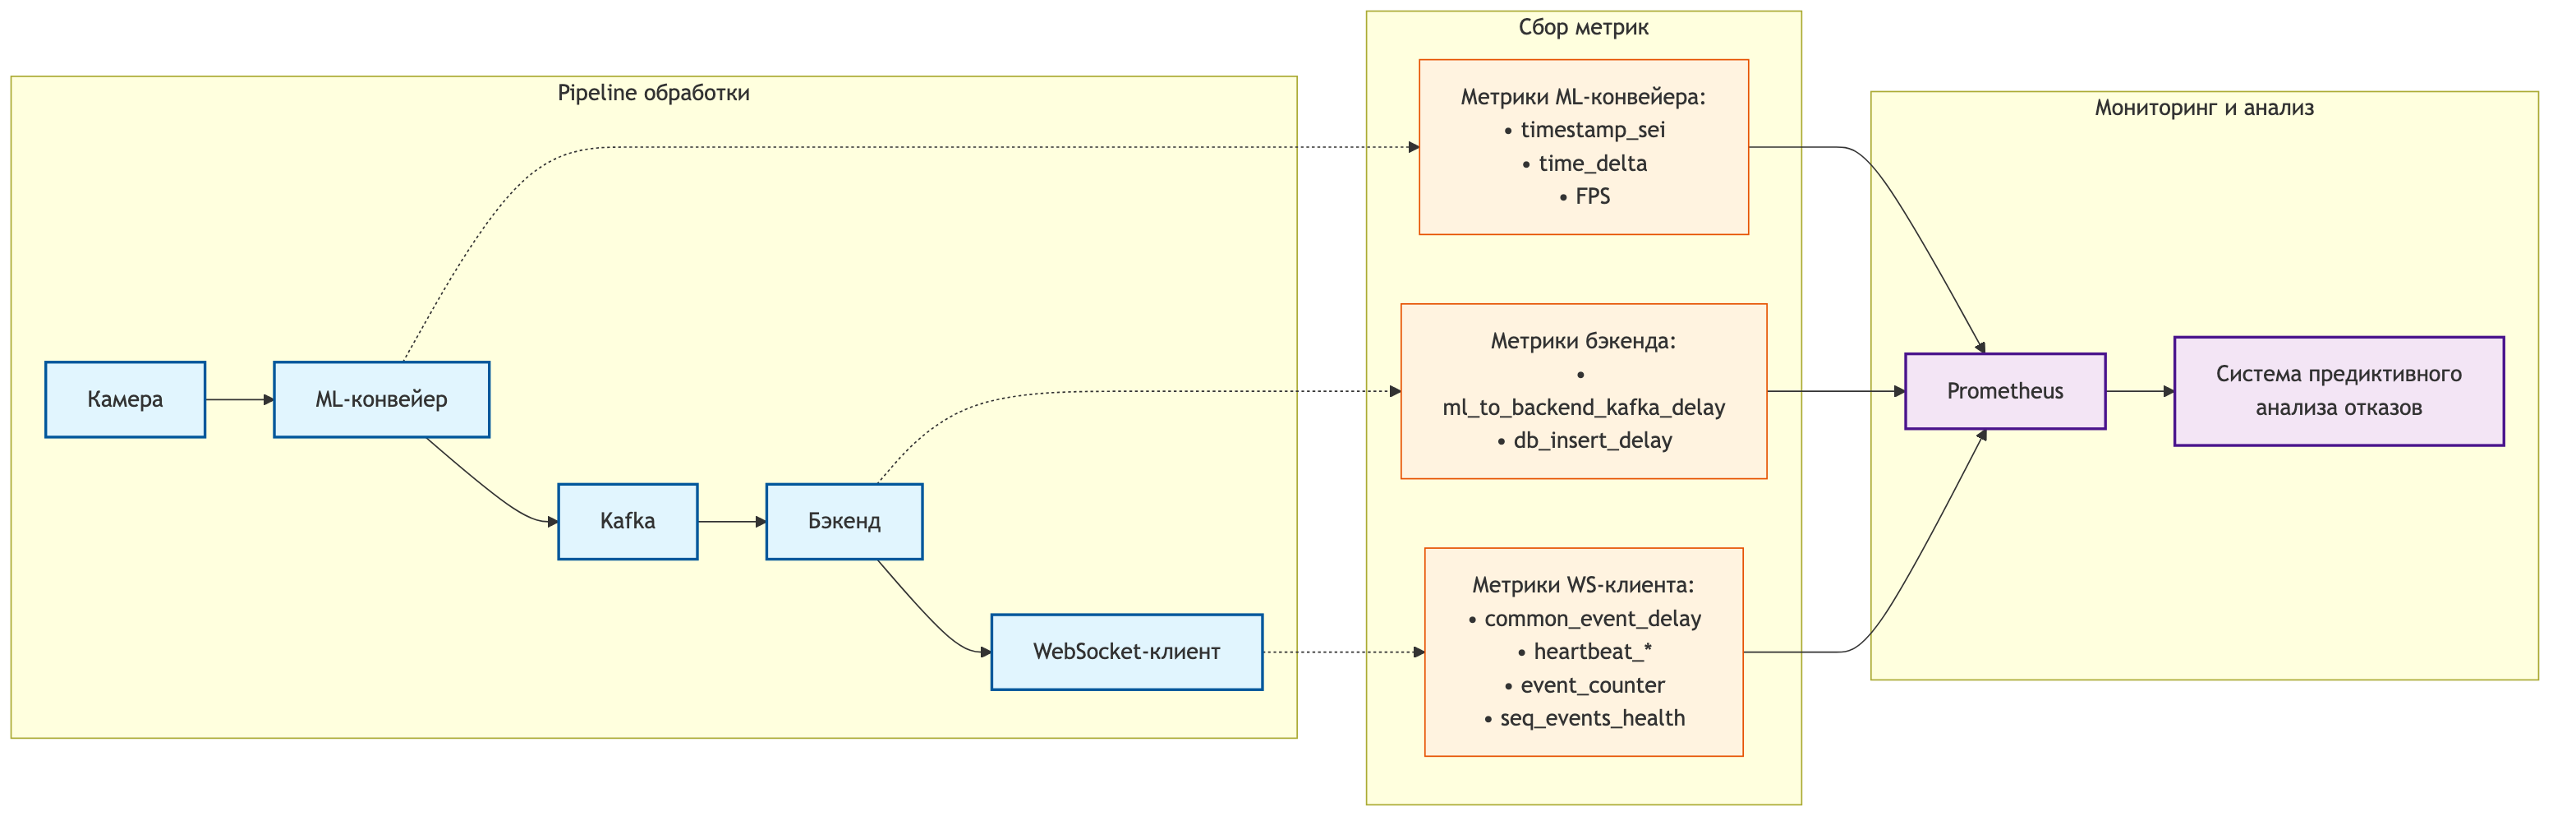
\includegraphics[width=\linewidth,height=\textheight,keepaspectratio]{figures/chapter1/video_pipeline_diagram.png}
	\caption*{Рисунок~1.1 --- Схема видеоконвейера и точки сбора метрик}
	\label{fig:video_pipeline}
\end{figure}
\vspace*{\fill}
\end{landscape}
